% Source : http://tex.stackexchange.com/questions/30032/highlighting-diagonal-of-a-square-matrix

\documentclass{article}
	\usepackage{tikz}
	\usetikzlibrary{matrix,shapes}


\begin{document}

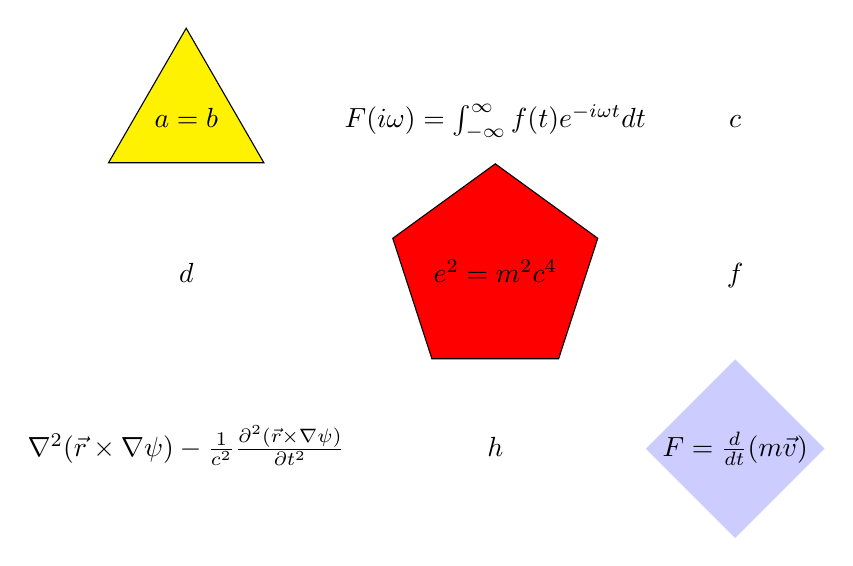
\begin{tikzpicture}
\matrix (m) [matrix of math nodes,inner sep=0cm]{
	| [draw,regular polygon,regular polygon sides=3,fill= yellow] 
	| a=b&F(i\omega) = \int^{\infty}_{-\infty}f(t)e^{-i\omega t}dt &c \\
%Second row
	d&
	|[draw,regular polygon,fill= red]
	| e^2=m^2c^4 &f\\
%Third row
	\nabla^2(\vec{r}\times \nabla\psi)  - \frac{1}{c^2}\frac{\partial^2 (\vec{r}\times \nabla\psi)}{\partial t^2}&h&|[diamond,fill= blue!20]|F = \frac{d}{dt}{(m\vec{v})}\\
};
\end{tikzpicture}

\end{document}
